\documentclass[11pt, oneside]{article}   	% use "amsart" instead of "article" for AMSLaTeX format
\usepackage{geometry}                		% See geometry.pdf to learn the layout options. There are lots.

\usepackage{tabularx}           % For creating tables with auto-wrapping text columns
\geometry{letterpaper, top=1in, bottom=1in}                          		% ... or a4paper or a5paper or ... 
%\geometry{landscape}                		% Activate for rotated page geometry
\usepackage[parfill]{parskip}    			% Activate to begin paragraphs with an empty line rather than an indent 
\usepackage{graphicx}				% Use pdf, png, jpg, or eps§ with pdflatex; use eps in DVI mode   
                                % TeX will automatically convert eps --> pdf in pdflatex. 
                                    
\usepackage{amssymb}
\usepackage{mathtools}
\usepackage{enumerate}
\usepackage{tikz}
% \usepackage[htt]{hyphenat} 
\usepackage[normalem]{ulem}
\usepackage{xcolor} % Required for colors
\usepackage[most]{tcolorbox} % Required for the answer boxes
\usepackage[T1]{fontenc}
\usepackage{lmodern}
\usepackage{microtype}


\usepackage{hyperref}
\usepackage{tcolorbox}
\tcbuselibrary{listings, skins, breakable}
%\usepackage[most]{tcolorbox} % Required for the answer boxes  
\usepackage{caption}
\usepackage{xparse}
\makeatletter
\newtcolorbox{answerbox}{
    enhanced,
    breakable,
    colback=yellow!10!white,
    colframe=gray!75!black,
    boxrule=0.8pt,
    arc=4pt,
    title=Answer:,
    coltitle=black,
    fonttitle=\bfseries,
    attach title to upper,
    after title={\par},
    valign=top,
    before upper={%
      % Save originals silently
      \let\abx@origfigure\figure
      \let\abx@endorigfigure\endfigure
      \let\abx@origtable\table
      \let\abx@endorigtable\endtable

      % Locally redefine figure
      \RenewDocumentEnvironment{figure}{ O{} }{%
        \captionsetup{type=figure}%
        \par\medskip\noindent\begin{center}\begin{minipage}{\linewidth}%
      }{%
        \end{minipage}\end{center}\par\medskip
      }

      % Locally redefine table
      \RenewDocumentEnvironment{table}{ O{} }{%
        \captionsetup{type=table}%
        \par\medskip\noindent\begin{center}\begin{minipage}{\linewidth}%
      }{%
        \end{minipage}\end{center}\par\medskip
      }
    },
    after upper={%
      % Restore originals when leaving the box
      \let\figure\abx@origfigure
      \let\endfigure\abx@endorigfigure
      \let\table\abx@origtable
      \let\endtable\abx@endorigtable
    },
}
\makeatother


\newcommand{\ck}[1]{\textcolor{cyan}{CK: #1}}
\newcommand{\jc}[1]{\textcolor{blue}{JC: #1}}
\newcommand{\sss}[1]{\textcolor{magenta}{SS: #1}}
\newcommand{\ya}[1]{\textcolor{orange}{YA: #1}}
\newcommand{\yy}[1]{\textcolor{green}{YY: #1}}

\title{Homework 1 \\ CSC 277 / 477 \\ End-to-end Deep Learning \\ Fall 2025}
\author{John Doe - \texttt{jdoe@ur.rochester.edu}}
\date{}					

\begin{document}

\maketitle

\begin{center}
    \textbf{Deadline:} See Blackboard    
\end{center}


\section*{Instructions}

Your homework solution must be typed and prepared in \LaTeX. It must be output to PDF format. To use \LaTeX, we suggest using \url{http://overleaf.com}, which is free.

Your submission must cite any references used (including articles, books, code, websites, and personal communications).  All solutions must be written in your own words, and you must program the algorithms yourself. \textbf{If you do work with others, you must list the people you worked with.} Submit your solutions as a PDF to Blackboard. 


Your programs must be written in Python. You will use \emph{PyTorch with Lightning Fabric} (\href{https://docs.pytorch.org/tutorials/beginner/basics/intro.html}{PyTorch}, \href{https://lightning.ai/docs/fabric/stable/}{Lightning Fabric}) in this homework. All deliverables should be within the answer box provided, i.e., \textbackslash begin\{answerbox\} DELIVERABLES \textbackslash end\{answerbox\}. If a problem requires code as a deliverable, then the code should be shown as part of the solution. One easy way to do this in \LaTeX \, is to use the verbatim environment, i.e., \textbackslash begin\{verbatim\} YOUR CODE \textbackslash end\{verbatim\}.



%%%%%%%%%%%%%%%%%%%%%%%%%%%%%%%%%%%%%%%%%%%%%
\paragraph{About Homework 1:} Homework 1 aims to acquaint you with hyperparameter tuning, network fine-tuning, WandB for Training Monitoring, and model testing. \emph{Keep in mind that network training is time-consuming, so begin early!} Copy and paste this template into an editor, e.g., \url{www.overleaf.com}, and then just type the answers in. You can use a math editor to make this easier, e.g., CodeCogs Equation Editor or MathType. \href{https://blog.writefull.com/texgpt-harness-the-power-of-chatgpt-in-overleaf/}{You may use the AI (LLM) plugin for Overleaf for help you with \LaTeX formatting.}

%CodeCogs: \url{https://www.codecogs.com/latex/eqneditor.php}

%MathType: \url{http://www.dessci.com/en/products/mathtype/}
%For MathType, you have to tell it to export as LaTex. 


\clearpage

\section*{Problem 1 - WandB for Training Monitoring}

Training neural networks involves exploring different model architectures, hyperparameters, and optimization strategies. Monitoring these choices is crucial for understanding and improving model performance. Logging experiment results during training helps to:
\begin{itemize}
    \item Gain insights into model behavior (e.g., loss, accuracy, convergence patterns).
    \item Optimize hyperparameters by evaluating their impact on stability and accuracy.
    \item Detect overfitting or underfitting and make necessary adjustments.
\end{itemize}

In this problem, you'll train ResNet-18 models for image classification on the \href{https://www.kaggle.com/datasets/tanlikesmath/the-oxfordiiit-pet-dataset?select=images}{Oxford-IIIT Pet Dataset} while exploring various hyperparameters. You’ll use \href{https://docs.wandb.ai/tutorials/experiments}{Weights and Biases (W\&B)} to log your experiments and refine your approach based on the results.

\subsection*{Part 1: Implementing Experiment Logging with W\&B (7 points)}

\noindent \textbf{Prepare the Dataset.} Download the \href{https://www.kaggle.com/datasets/tanlikesmath/the-oxfordiiit-pet-dataset?select=images}{dataset}. Complete the dataset definition in \texttt{train.py}. Make a custom \texttt{Dataset} class (\href{https://wandb.ai/sauravmaheshkar/Dataset-DataLoader/reports/An-Introduction-to-Datasets-and-DataLoader-in-PyTorch--VmlldzoxMDI5MTY2}{examples}, \href{https://docs.pytorch.org/vision/main/datasets.html}{reference}) or use \href{https://pytorch.org/vision/stable/generated/torchvision.datasets.ImageFolder.html}{\texttt{ImageFolder}} to do this. Use the splits defined in \texttt{oxford\_pet\_split.csv} to define the training, validation, and test splits. In the dataset's preprocessing, resize the images to $224$ as required by ResNet-18, and apply \href{https://discuss.pytorch.org/t/understanding-transform-normalize/21730}{image normalization} using \href{https://stackoverflow.com/questions/73350133/how-to-calculate-mean-and-standard-deviation-of-a-set-of-images}{statistics from the training set} or from \href{https://stackoverflow.com/questions/58151507/why-pytorch-officially-use-mean-0-485-0-456-0-406-and-std-0-229-0-224-0-2}{ImageNet}.

\noindent \textbf{Evaluating Model Performance.}
During model training, the validation set is a crucial tool to prevent overfitting. Complete \texttt{evaluate()} function in \texttt{train.py} which takes a model and a dataloader as inputs and outputs the model's accuracy score and cross-entropy loss on the dataset. 

\noindent \textbf{Integrate W\&B Logging.}
To integrate W\&B for experiment logging, follow these steps and add the necessary code to \texttt{train.py}:
\begin{enumerate}
    \item Refer to the W\&B \href{https://docs.wandb.ai/tutorials/experiments}{official tutorial} for guidance.
    \item Initialize a new run at the start of the experiment following the tutorial's code snippet. Log basic experiment \textbf{configurations}, such as total training epochs, learning rate, batch size, and scheduler usage. Ensure the run \textbf{name} is interpretable and reflects these key details.
    \item During training, log the training loss and learning rate after each mini-batch.
    \item After each epoch, log the validation loss and validation accuracy.
    \item At the end of the training, log the model's performance on the test set, including loss and accuracy scores.
\end{enumerate}

\noindent \textbf{Experiment and Analysis. }
Execute the experiment using the \textbf{default} setup (found in \texttt{get\_args} function). Log in to the W\&B website to inspect your implementation.

\noindent\textbf{Deliverable:}
\begin{itemize}
    \item Code snippet(s) completed to load the dataset.
    \item Screenshot(s) of the experiment configuration (\textit{Select the specific Run in W\&B, and then the Overview tab})
    \item Screenshot(s) of all logged charts (\textit{Select the specific Run in W\&B, and then Charts under Workspace tab}).
    \item Are the data logged accurately in the W\&B interface? Does the experiment configuration align with your expectations?
    \item Analyze the logged charts to determine whether the training has converged. 
\end{itemize}


\begin{answerbox} \textbf{Answer:} \vspace*{1cm}

    Code snippet(s) completed to load the dataset:
\begin{verbatim}
def build_split_dataset(dataset_root, selected_names, transform):
    dataset = ImageFolder(root=dataset_root, transform=transform)
    filtered_samples = [
        (path, target)
        for path, target in dataset.samples
        if Path(path).name in selected_names
    ]
    filtered_samples.sort(key=lambda entry: Path(entry[0]).name)
    dataset.samples = filtered_samples
    dataset.imgs = filtered_samples
    dataset.targets = [target for _, target in filtered_samples]
    return dataset
dataset_root = Path(__file__).resolve().parents[1] / "data"
metadata_path = Path(__file__).resolve().parent / "oxford_pet_split.csv"
metadata_frame = pl.read_csv(metadata_path)
train_names = set(
    metadata_frame.filter(pl.col("split") == "train")
    .get_column("image_name")
    .to_list()
)
val_names = set(
    metadata_frame.filter(pl.col("split") == "val")
    .get_column("image_name")
    .to_list()
)
test_names = set(
    metadata_frame.filter(pl.col("split") == "test")
    .get_column("image_name")
    .to_list()
)
normalization_mean = [0.485, 0.456, 0.406]
normalization_std = [0.229, 0.224, 0.225]

train_transforms = transforms.Compose([
    transforms.Resize((224, 224)),
    transforms.RandomHorizontalFlip(p=0.5),
    transforms.ToTensor(),
    transforms.Normalize(
        mean=normalization_mean, std=normalization_std),
])
eval_transforms = transforms.Compose([
    transforms.Resize((224, 224)),
    transforms.ToTensor(),
    transforms.Normalize(
        mean=normalization_mean, std=normalization_std),
])

train_set = build_split_dataset(
    dataset_root, train_names, train_transforms)
val_set = build_split_dataset(
    dataset_root, val_names, eval_transforms)
test_set = build_split_dataset(
    dataset_root, test_names, eval_transforms)
\end{verbatim}

Screenshot(s) of the experiment configuration:

\begin{figure}[h]
    \centering
    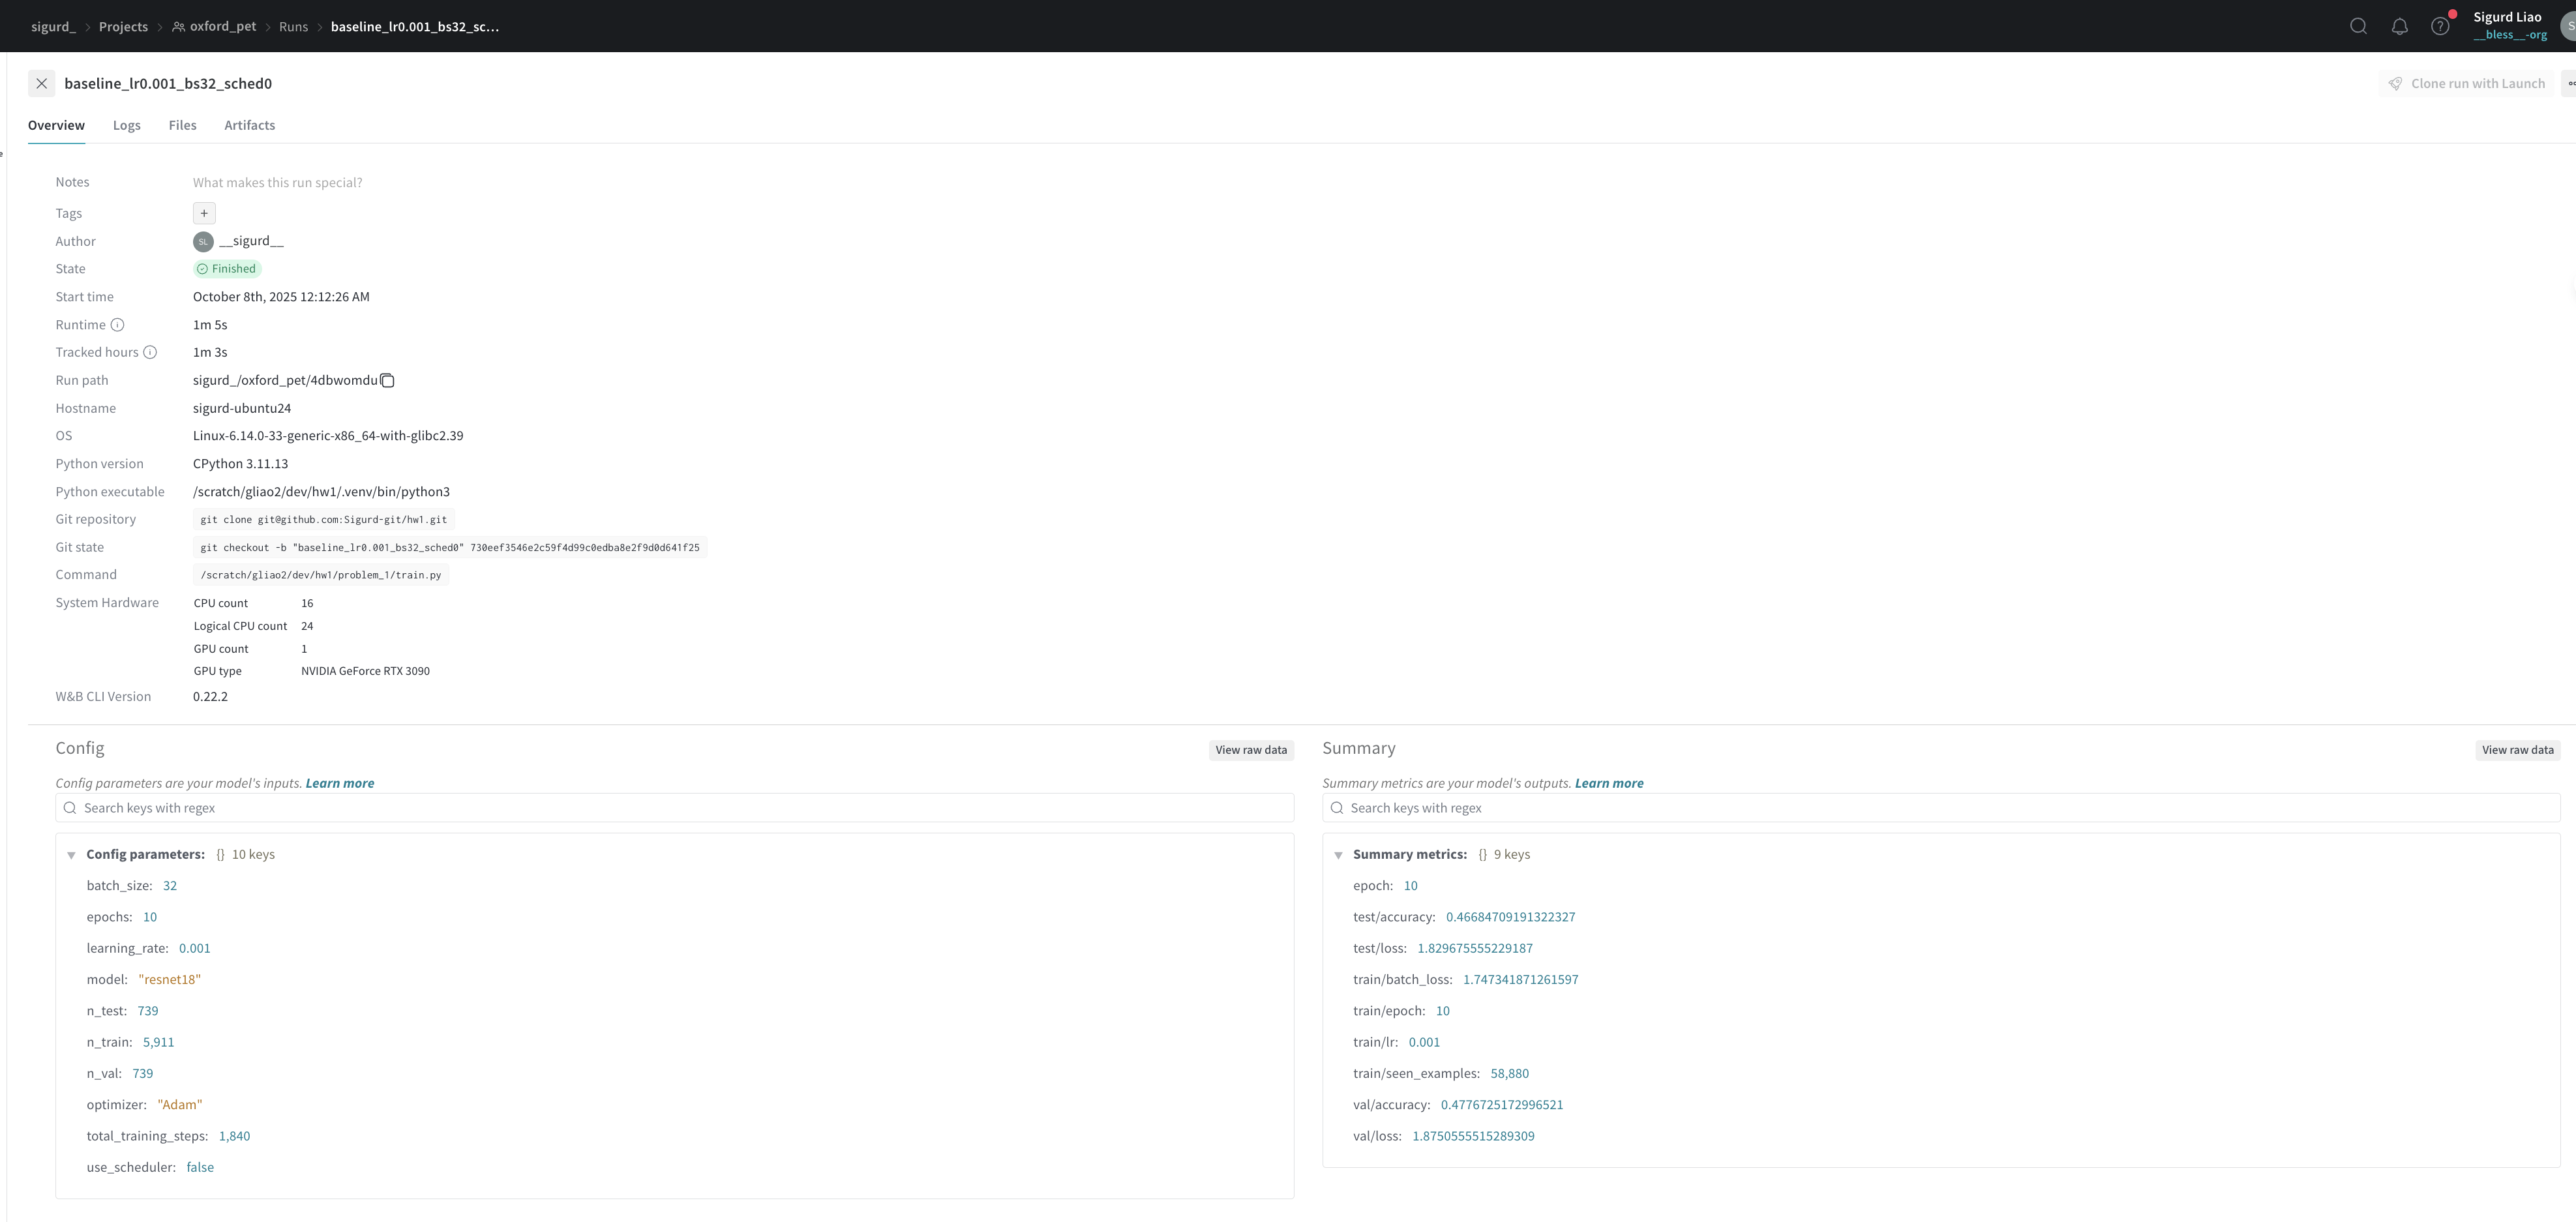
\includegraphics[width=0.8\textwidth]{images/experiment_configuration.png}
    \caption{Experiment Configuration}
\end{figure}

Screenshot(s) of all logged charts:

\begin{figure}[h]
    \centering
    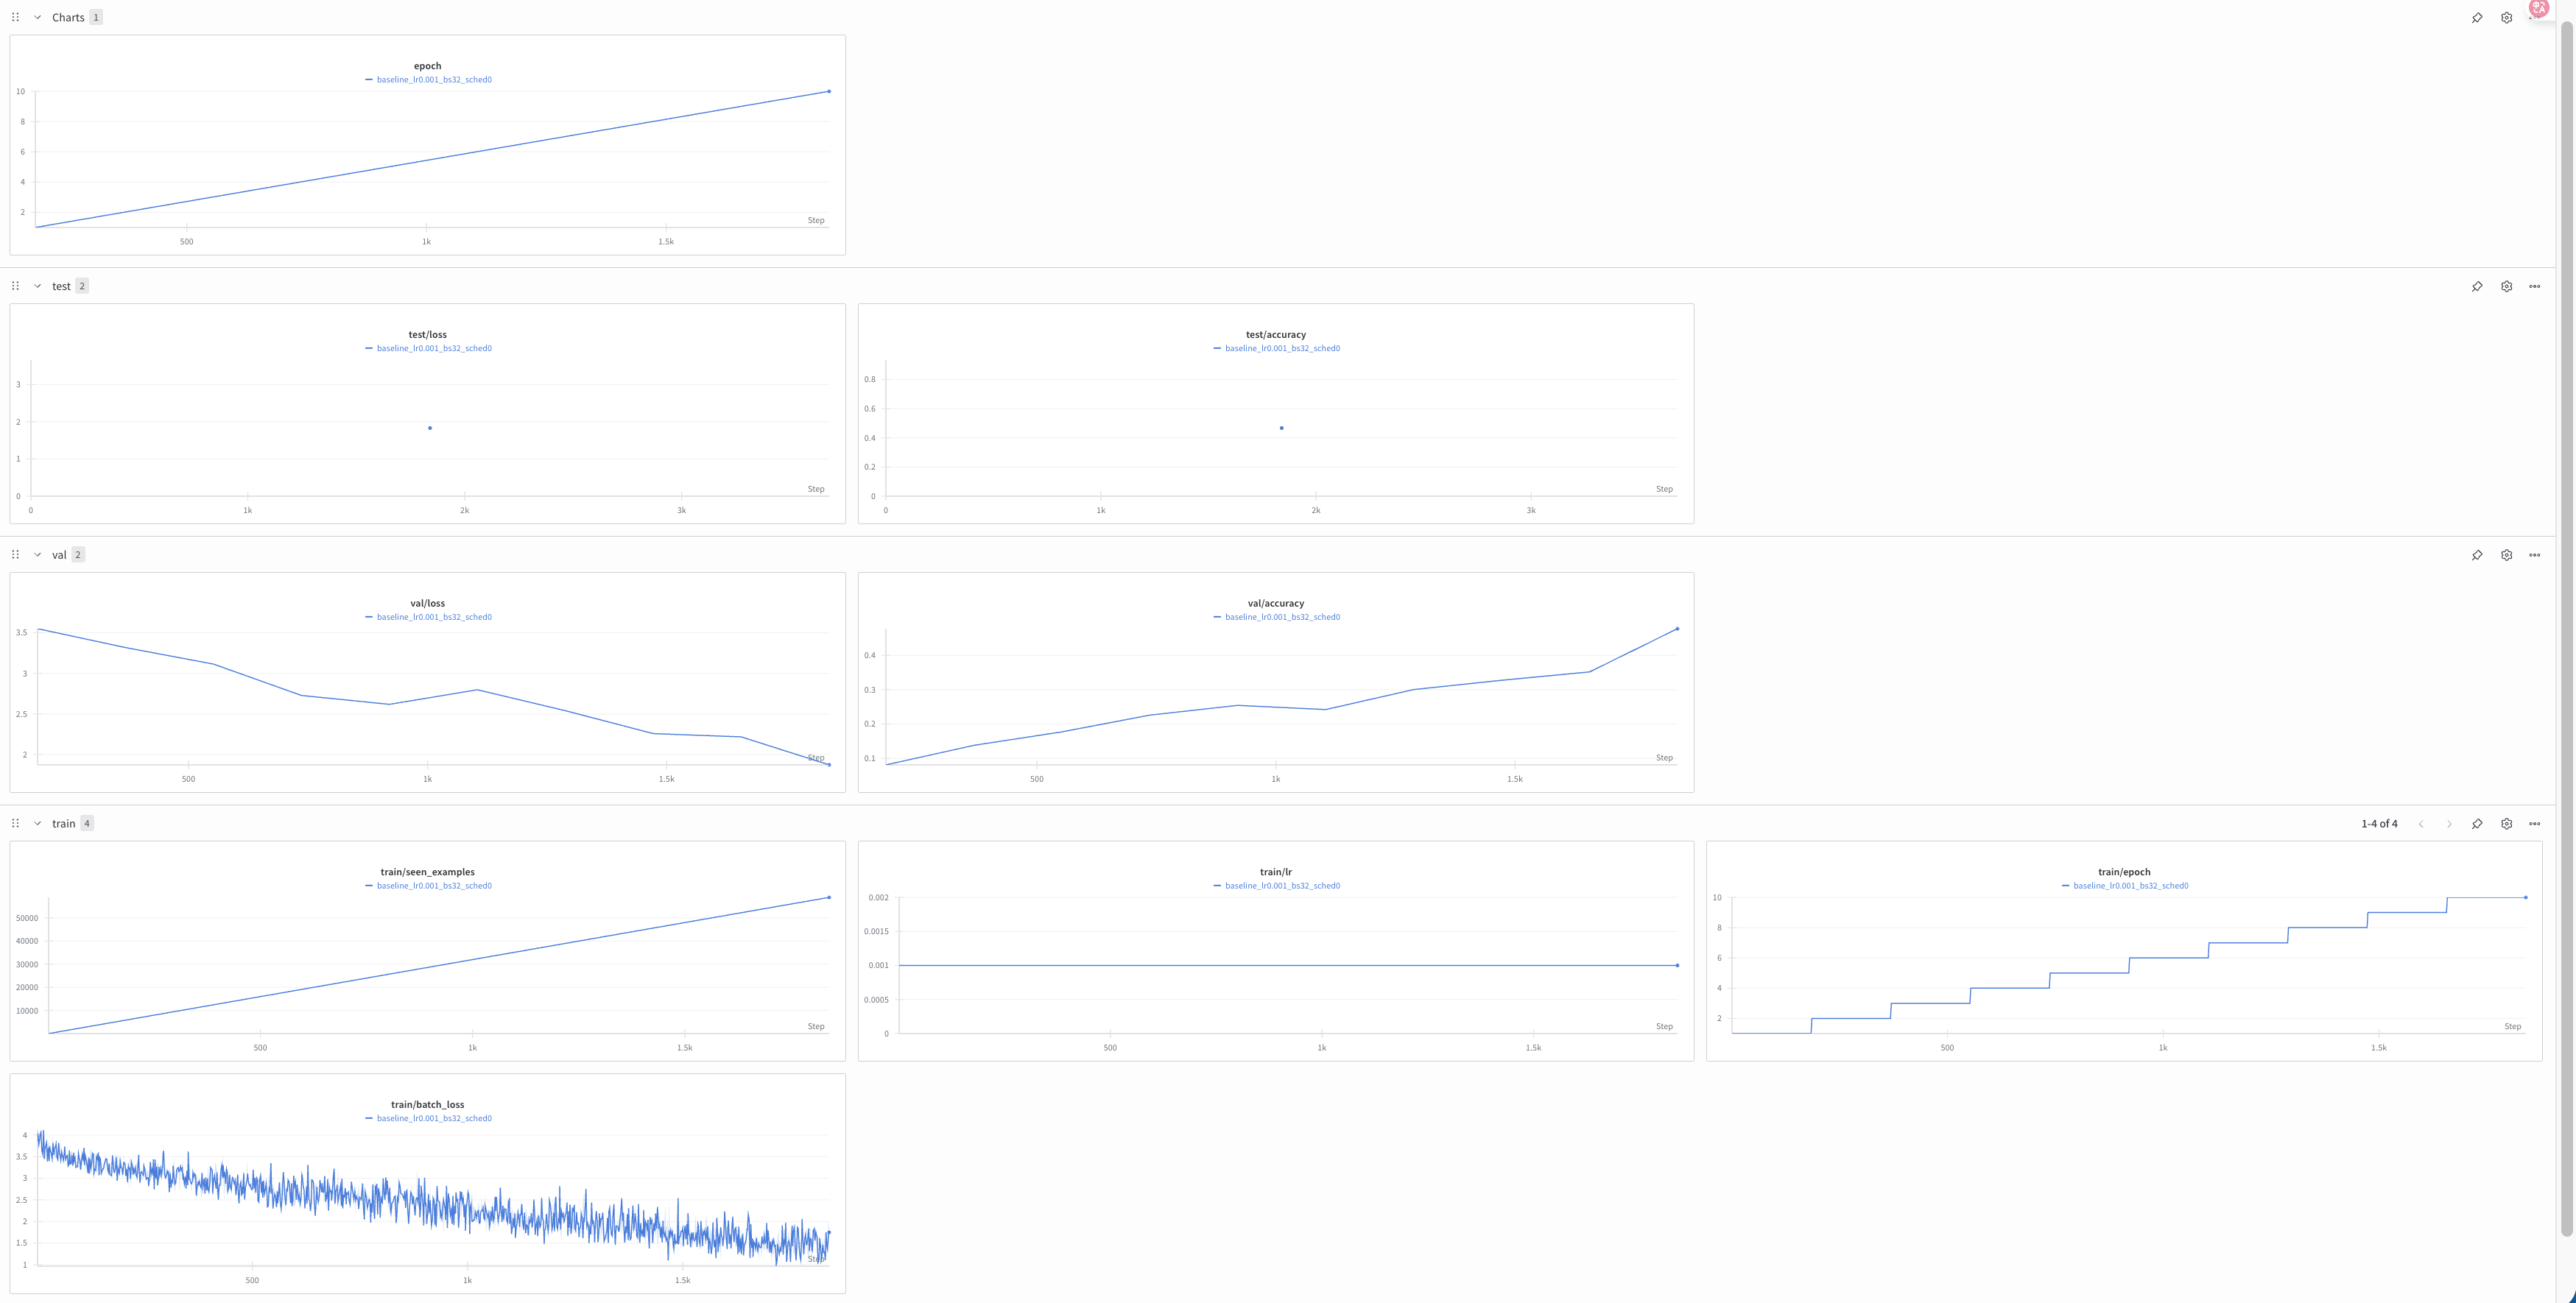
\includegraphics[width=0.8\textwidth]{images/logged_charts.png}
    \caption{Logged Charts}
\end{figure}


Data logged accurately in the W\&B interface? Does the experiment configuration align with your expectations?

Yes, the data is logged accurately in the W\&B interface. The experimental configuration aligns with my expectations, as both training and validation losses are decreasing and validation accuracy is increasing.

Analyze the logged charts to determine whether the training has converged.

The training has not converged yet since the losses are still decreasing and the validation accuracy is increasing.

\end{answerbox}


\subsection*{Part 2: Tuning Hyperparameters}
In this section, you'll experiment with key hyperparameters like learning rate and scheduler, and study their effects on training dynamics. For each step, change only one configuration at a time. Try not modify other hyperparameters (except batch size, which can be adjusted based on your computing resources).

\subsubsection*{Learning Rate Tuning with Sweep (5 points)}
 The learning rate is a crucial hyperparameter that significantly affects model convergence and performance.  Run the training script using \href{https://docs.wandb.ai/guides/sweeps/walkthrough}{W\&B sweep} with the following learning rates: $1e-2$, $1e-4$, and $1e-5$. Also, include the default learning rate ($1e-3$) from Part 1 in your analysis.

\noindent\textbf{Deliverable:}
\begin{itemize}
    \item Provide screenshots of logged charts showing learning rate, training loss, validation accuracy, and final test accuracy. Each chart should display results from \textbf{multiple runs} (all four learning rates in one chart). Ensure that titles and legends are clear and easy to interpret.
    \item Analyze how the learning rate impacts the training process and final performance.
    \item Code of your \href{https://docs.wandb.ai/guides/sweeps/define-sweep-configuration}{sweep configuration} that defines the search space.
\end{itemize}

\begin{answerbox} \textbf{Answer:} \vspace*{1cm}

Run Learning Rate vs Training Loss plot:

\begin{figure}[h]
    \centering
    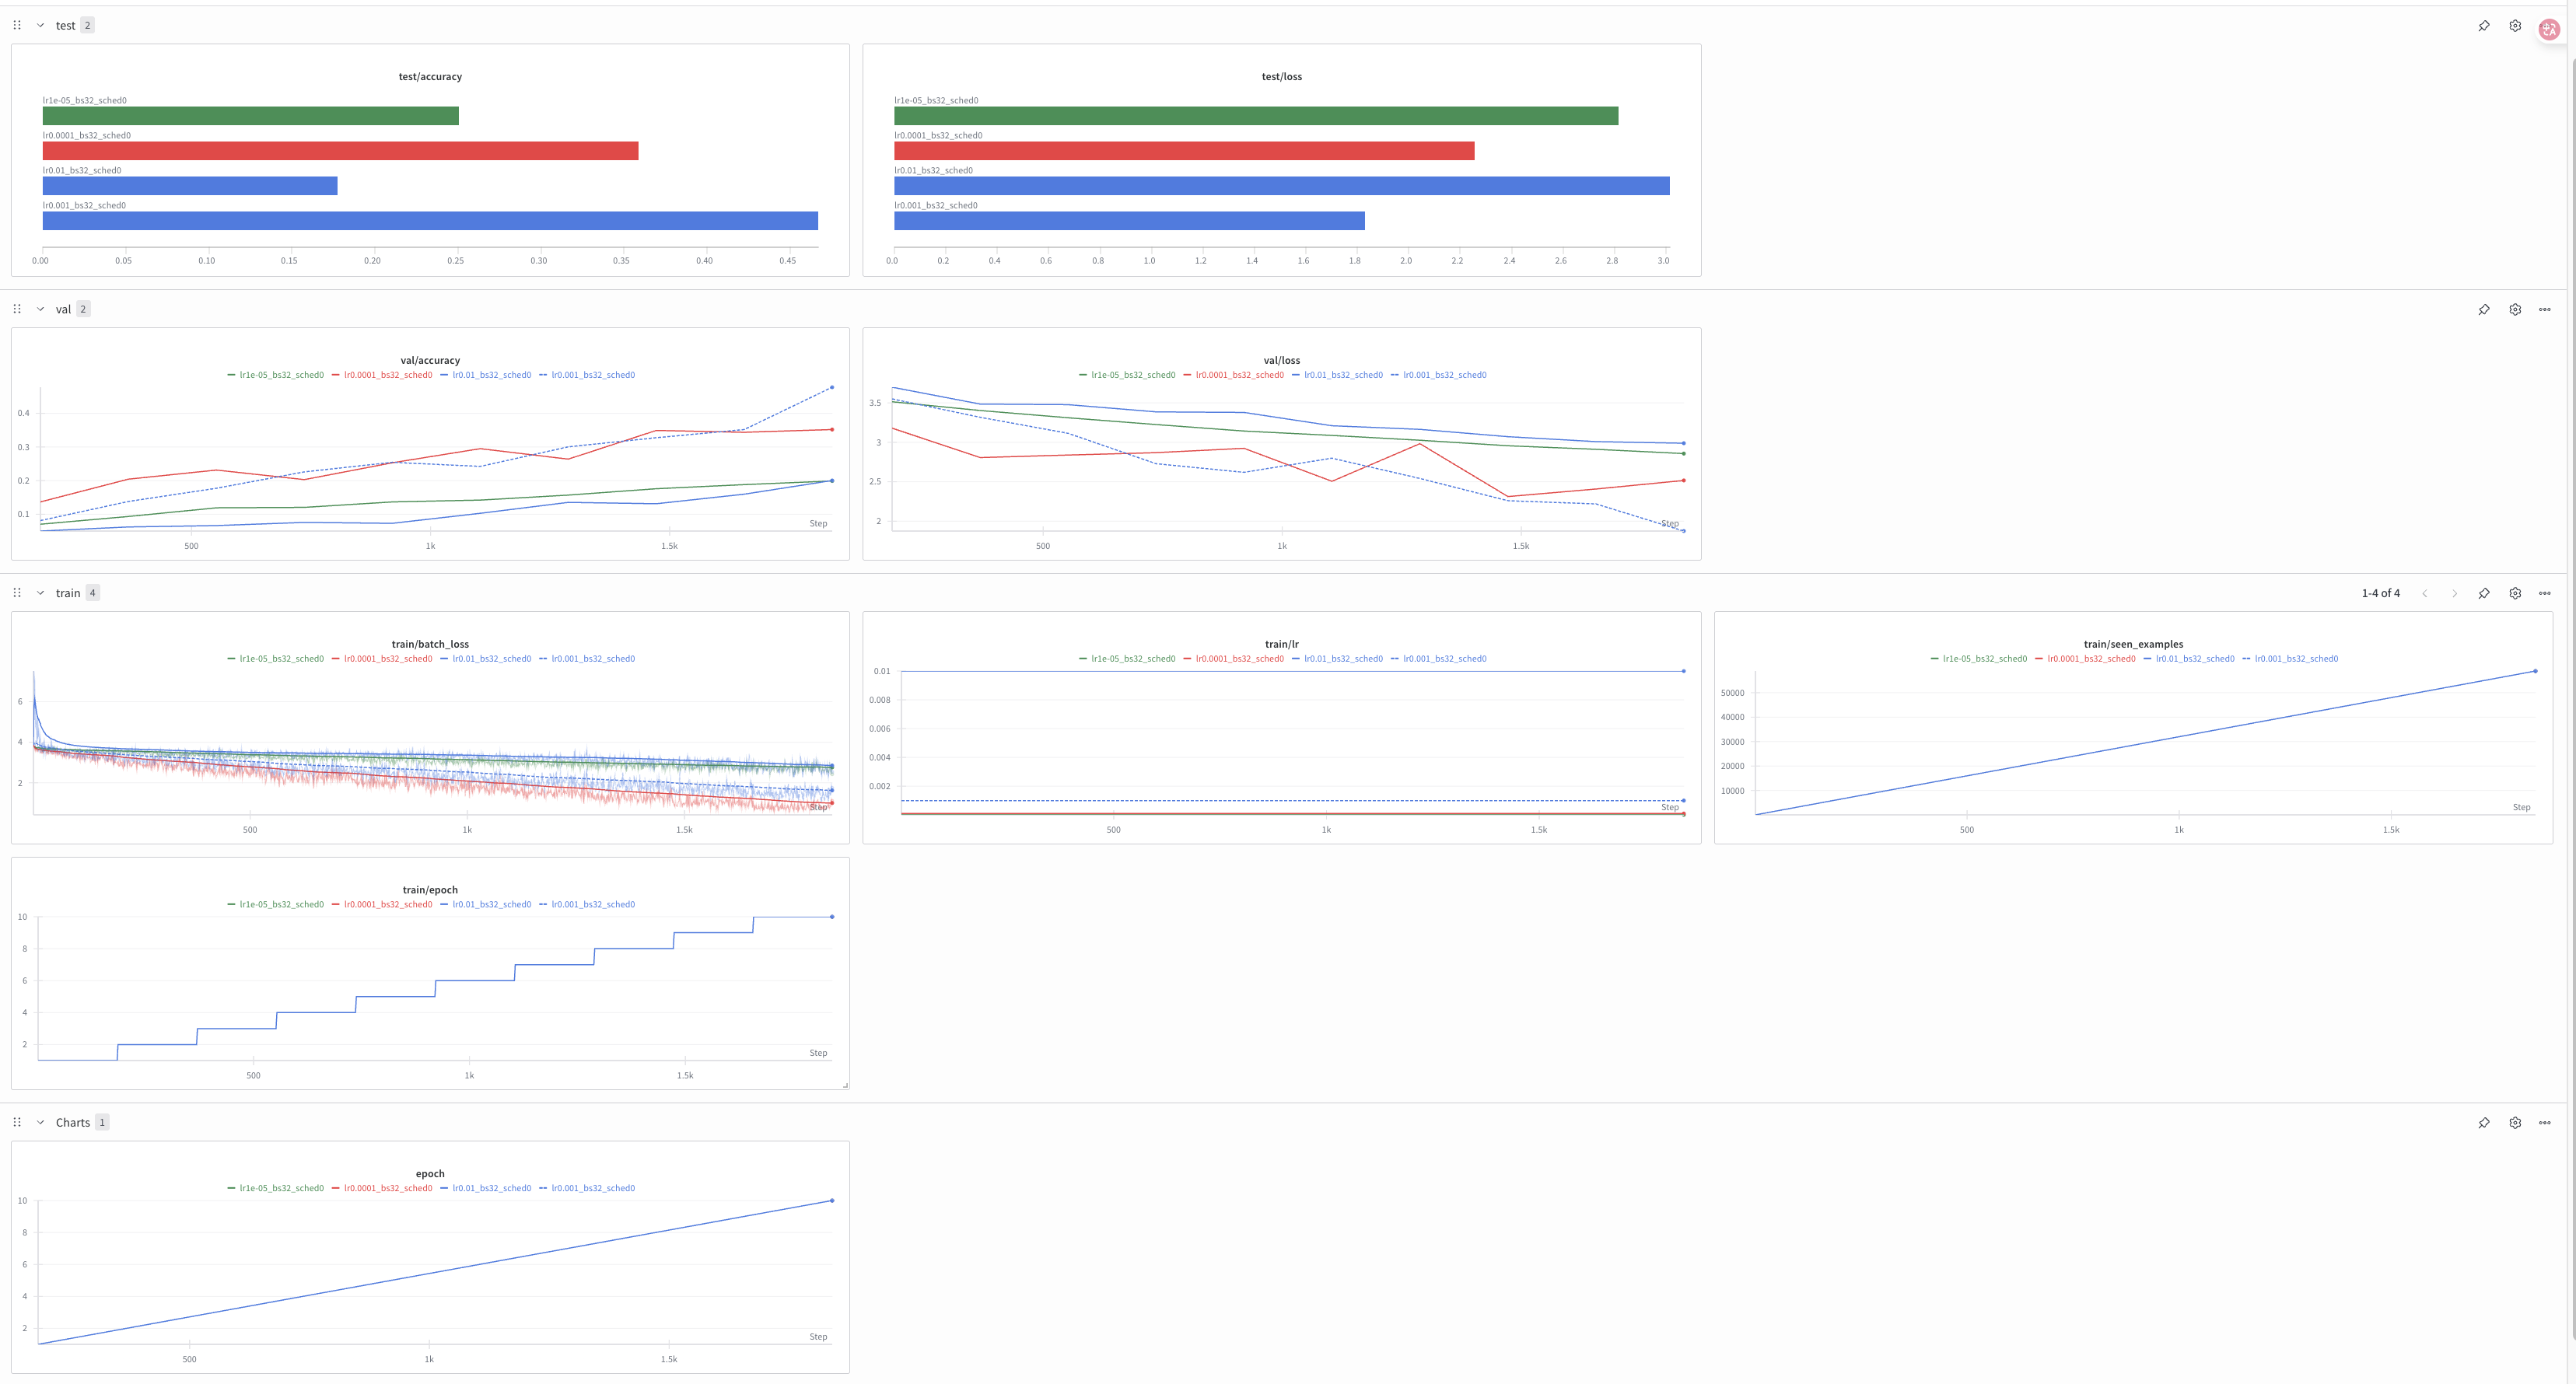
\includegraphics[width=0.8\textwidth]{images/lr.png}
    \caption{Learning Rate Impact}
\end{figure}

In theory, because the model has not yet converged, a relatively large learning rate might make the model perform better. However, as can be seen from the graph, when lr=0.001, there is the lowest val/test loss and the highest val/test accuracy. This indicates that an excessively large learning rate (0.01) may prevent the model from staying near a local optimum and instead jump out of the local optimum, leading to performance degradation. If you want to pursue extreme performance, you can try setting a finer grid between 0.01 and 0.0001. But I believe this is not the key to improving performance. Since the model has not yet converged, what we should do is increase the number of epochs. In addition, lr=0.001 or 0.0001 allows the model to converge the fastest. In conclusion, I believe that the default 0.001 is already a relatively reasonable choice.

Code of your \href{https://docs.wandb.ai/guides/sweeps/define-sweep-configuration}{sweep configuration} that defines the search space:

\begin{verbatim}
    program: problem_1/train.py
    method: grid 
    metric:
      name: val/loss
      goal: minimize
    parameters:
      lr:
        values: [1e-2, 1e-4, 1e-5]
\end{verbatim}

\end{answerbox}

\subsubsection*{Gradient Norm Monitoring for Exploding/Vanishing Gradients (4 points)}
Monitoring gradient norms during training is essential to detect exploding gradients (leading to instability or NaN losses) or vanishing gradients (causing slow/no convergence), which are common critical issues in deep learning practice. In \texttt{train.py}, extend your W\&B logging to compute and log the average L2 gradient norm across all model parameters after each batch (e.g., via a loop over \texttt{model.parameters()}). Run a `problematic' variant (e.g., set learning rate to 0.1 or larger values to induce exploding gradients). Compare the norm charts and loss curves of the problematic variant and your default run.

\noindent\textbf{Deliverable:}
\begin{itemize}
\item Screenshots of W\&B charts showing gradient norms and training loss over steps for both runs.
\item Do you notice signs of exploding/vanishing gradients in the problematic run? If so, identify them and explain your inferences. 
\item Code snippet(s) to compute and log gradient norms.
\end{itemize}
\textbf{Hint:} Consider carefully the placement of the Gradient norm calculation in the training loop's backward pass.

\begin{answerbox} \textbf{Answer:} \vspace*{1cm}

Screenshots of W\&B charts showing gradient norms and training loss over steps for both runs:

\begin{figure}[h]
    \centering
    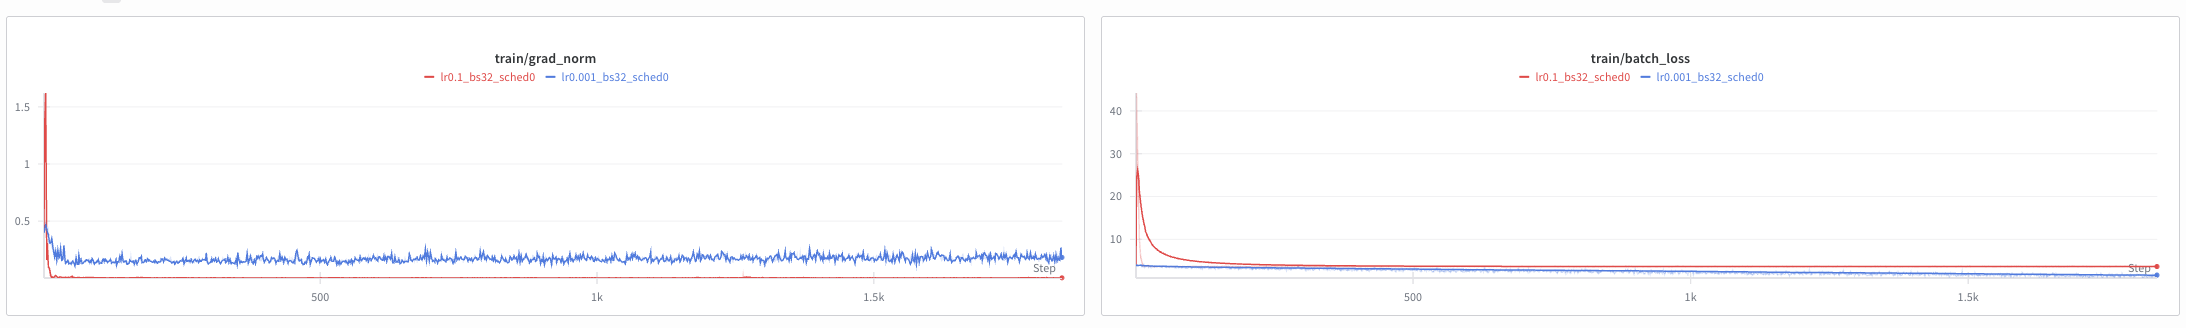
\includegraphics[width=0.8\textwidth]{images/grad_norm.png}
    \caption{Gradient Norm}
\end{figure}

Do you notice signs of exploding/vanishing gradients in the problematic run? If so, identify them and explain your inferences.

Yes, I noticed the gradient explosion. From the graph, it can be seen that when lr=0.1, the gradient explosion is very severe, with the gradient norm rapidly rising to more than three times that at r=0.001, and then quickly dropping to 0. Meanwhile, the train loss rapidly increases and suddenly drops, then remains at a relatively low value. I noticed that the accuracy of val is almost a straight line and does not change, while the accuracy of the test is about 0.025. I did not calculate the accuracy of random guessing, but I suspect that the reason it remains stable might be because the excessively large learning rate disrupts the distribution of the model's parameters, causing the model to almost guess randomly.

Code snippet(s) to compute and log gradient norms:

\begin{verbatim}
if fabric.is_global_zero: # Used to operate only on the main process (if distributed training is used)
    current_lr = optimizer.param_groups[0]["lr"]
    parameter_norms = [
        parameter.grad.detach().norm(2)
        for parameter in model.parameters()
        if parameter.grad is not None
    ]
    average_gradient_norm = torch.stack(parameter_norms).mean().item() if parameter_norms else 0.0
    batch_metrics = {
        "train/batch_loss": float(loss.item()),
        "train/lr": current_lr,
        "train/epoch": epoch,
        "train/seen_examples": seen_examples,
        "train/grad_norm": average_gradient_norm,
    }
    if wandb_run is not None:
        wandb.log(batch_metrics, step=global_step)
\end{verbatim}

\end{answerbox}

\subsubsection*{Learning Rate Scheduler (4 points)}

Learning rate schedulers dynamically adjust the learning rate during training, improving efficiency, convergence, and overall performance. In this step, you'll implement the \texttt{OneCycleLR} scheduler in the \texttt{get\_scheduler()} function within \texttt{train.py}. Compare the results to the baseline (default setting). If implemented correctly, the learning rate will initially increase and then decrease during training.

\noindent\textbf{Deliverable:}
\begin{itemize}
    \item Provide charts comparing the new setup with the baseline: learning rate, training loss, validation accuracy, and final test accuracy.
    \item Explain how the \texttt{OneCycleLR} scheduler impacts the learning rate, training process, and final performance compared to the baseline.
\end{itemize}

\begin{answerbox} \textbf{Answer:} \vspace*{1cm}


Screenshot(s) of W\&B charts:

\begin{figure}[h]
    \centering
    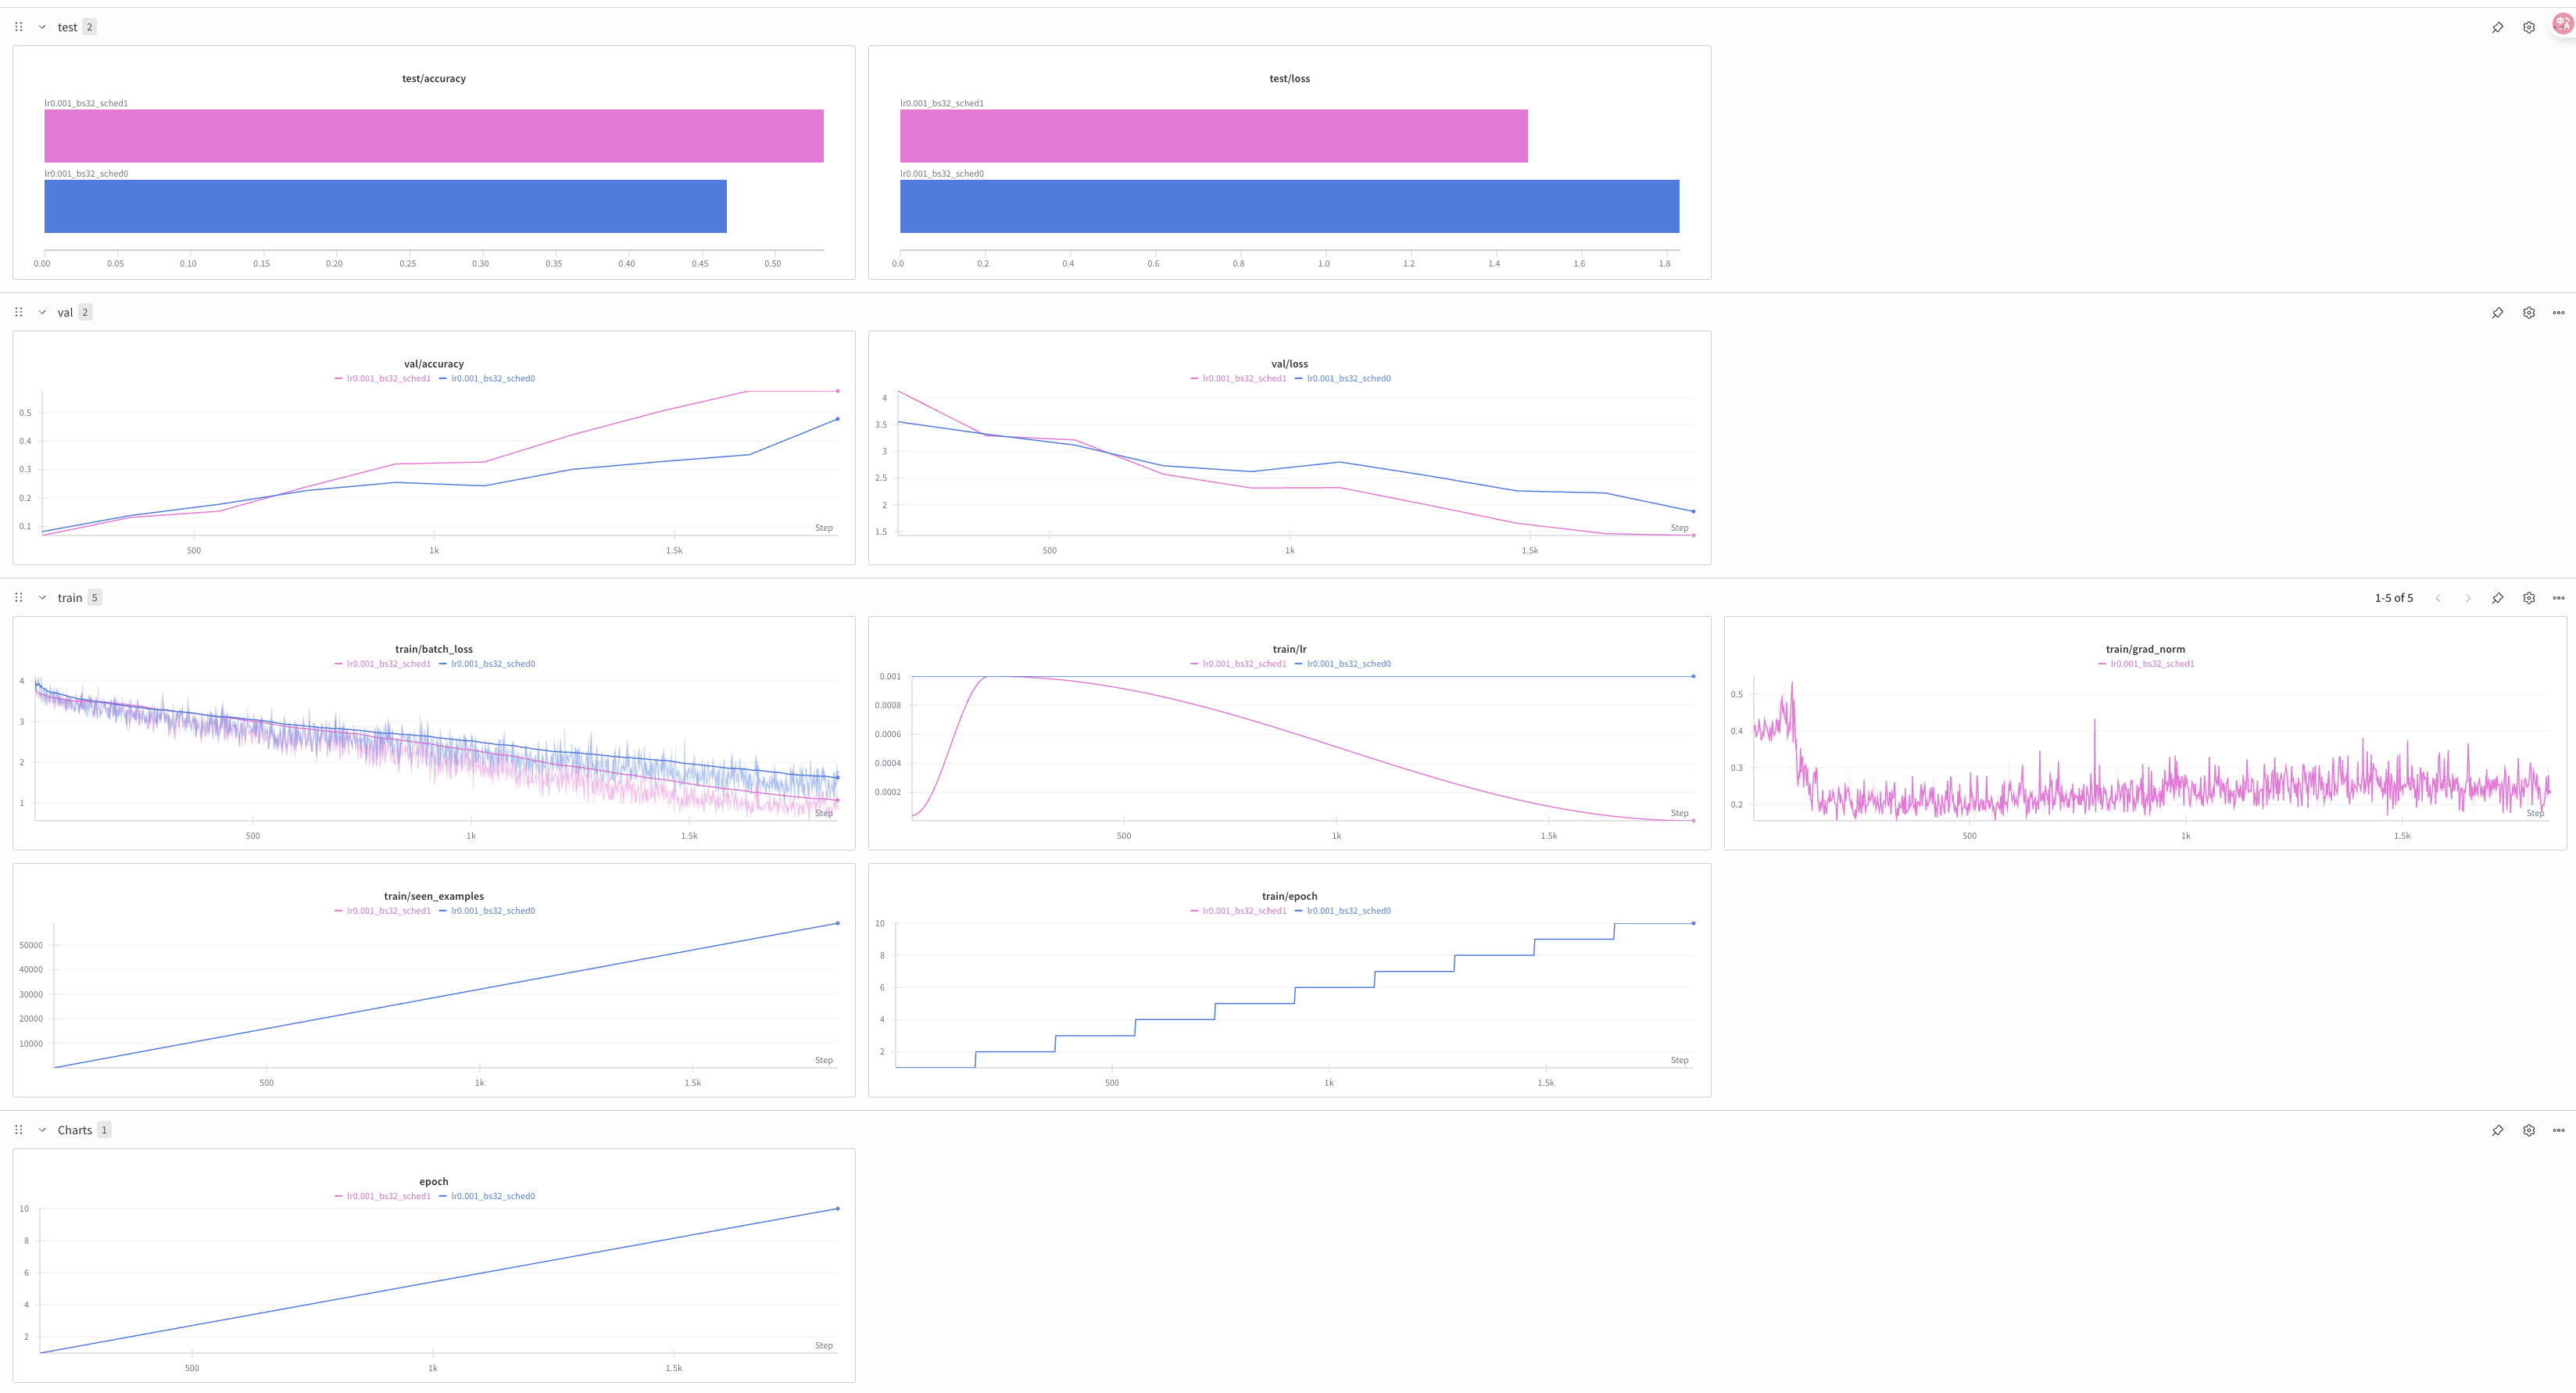
\includegraphics[width=0.8\textwidth]{images/scheduler.png}
    \caption{Learning Rate Scheduler}
\end{figure}

\texttt{OneCycleLR} scheduler allows the learning rate to first rise and then fall, which helps the model remain stable in the early stages of training (preventing gradient explosion due to an excessively high learning rate) and converge quickly in the later stages (because reducing the learning rate after reaching near a local optimum makes it easier for the model to achieve a local optimum). The final results show that with a scheduler, the validation loss decreases faster, and the final loss is also smaller. The validation accuracy increases faster, and the final result is higher. On the test set, the accuracy with a scheduler is also higher, and the loss is lower. Overall, the effect of the scheduler is positive.


\end{answerbox}



\subsection*{Part 3: Scaling Learning Rate with Batch Size (4 points)}

As observed in previous parts, the choice of learning rate is crucial for effective training. As batch size increases, the effective step size in the parameter space also increases, requiring adjustments to the learning rate. In this section, you'll investigate how to scale the learning rate appropriately when the batch size changes. Read the first few paragraphs of \href{https://www.cs.princeton.edu/~smalladi/blog/2024/01/22/SDEs-ScalingRules/}{this blog post} to understand scaling rules for Adam (used in default) and SGD optimizers. Then, conduct experiments to verify these rules. First, double (or halve) the batch size without changing the learning rate and run the training script. Next, ONLY adjust the learning rate as suggested in the post. Compare these results with the default setting. Note that since the total training steps vary with batch size, you should also log the number of seen examples to create accurate charts for comparison.


\noindent\textbf{Deliverable:}
\begin{itemize}
    \item Present charts showing: training loss and validation accuracy (with the x-axis being \texttt{seen\_examples}), and final test accuracy. Ensure the legends are clear. You may apply smoothing for better visualization. 
    \item Analyze the results: do they align with the patterns discussed in the blog post?
\end{itemize}

\begin{answerbox} \textbf{Answer:} \vspace*{1cm}


Screenshot(s) of W\&B charts:

\begin{figure}[h]
    \centering
    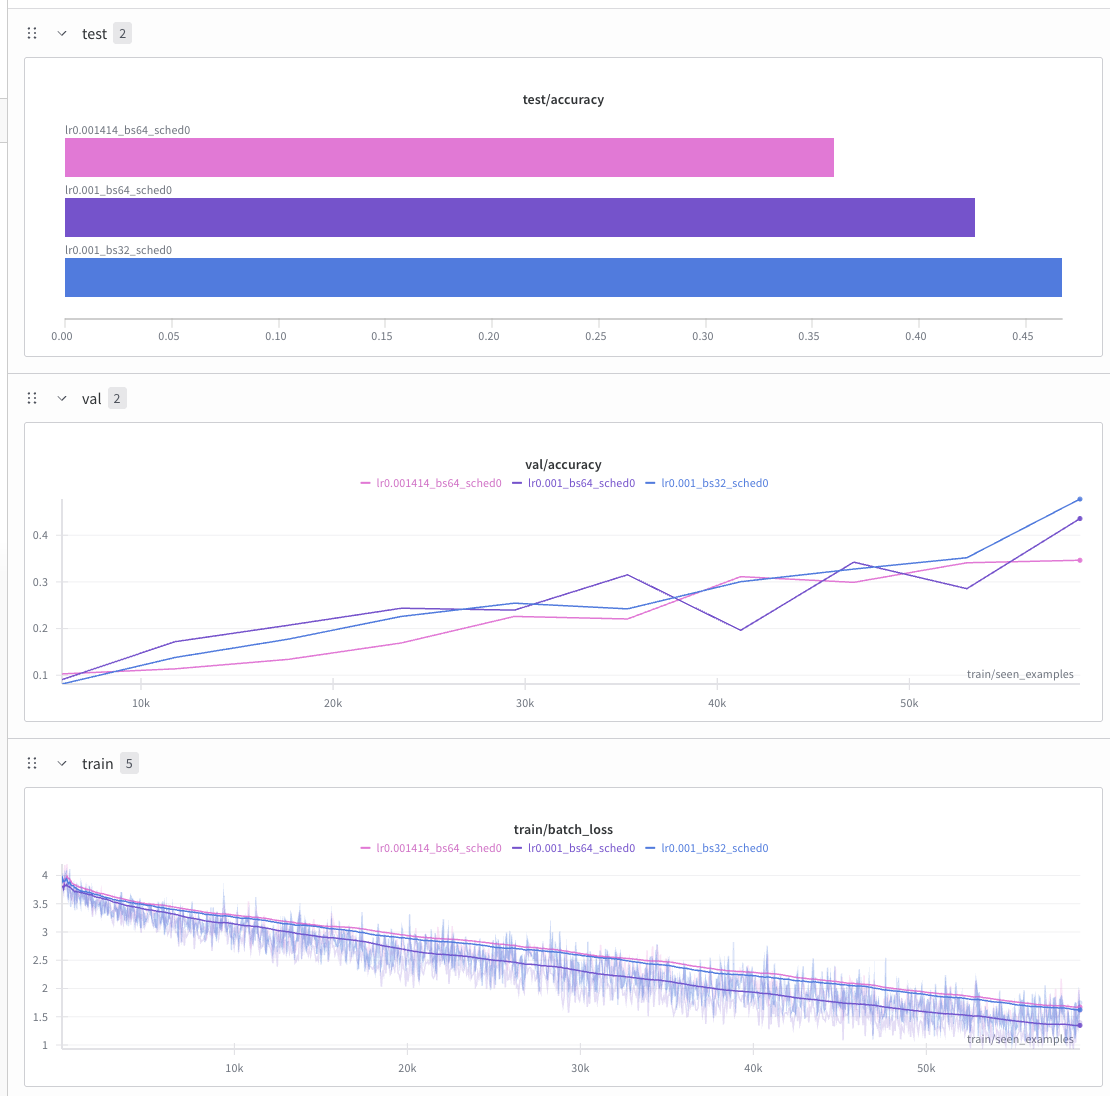
\includegraphics[width=0.8\textwidth]{images/batch_size.png}
    \caption{Batch Size}
\end{figure}

Their pattern does not match the blog post. According to the blog post, when the batch size increases, the learning rate should increase. Since we are using Adam, the learning rate should increase by the square root of 2 times. However, in reality, after increasing the learning rate by the square root of 2 times, I did not see better validation and test accuracy compared to the default learning rate. I think there could be multiple factors; firstly, the model has not yet converged, and perhaps after convergence, the effect might be different. Secondly, these rules are just a theoretical optimal solution and can easily vary with different datasets and models.

To verify my first hypothesis, I added a scheduler for all three conditions. Based on previous attempts, I know that with a scheduler, the model converges better than without one, and in the later stages of training, the validation loss decreases very slowly, almost leveling off. However, in this case, the condition with the increased learning rate still does not outperform the condition with the default learning rate. Therefore, although it is unfortunate, this assignment does not match the pattern described in the blog.

\begin{figure}[h]
    \centering
    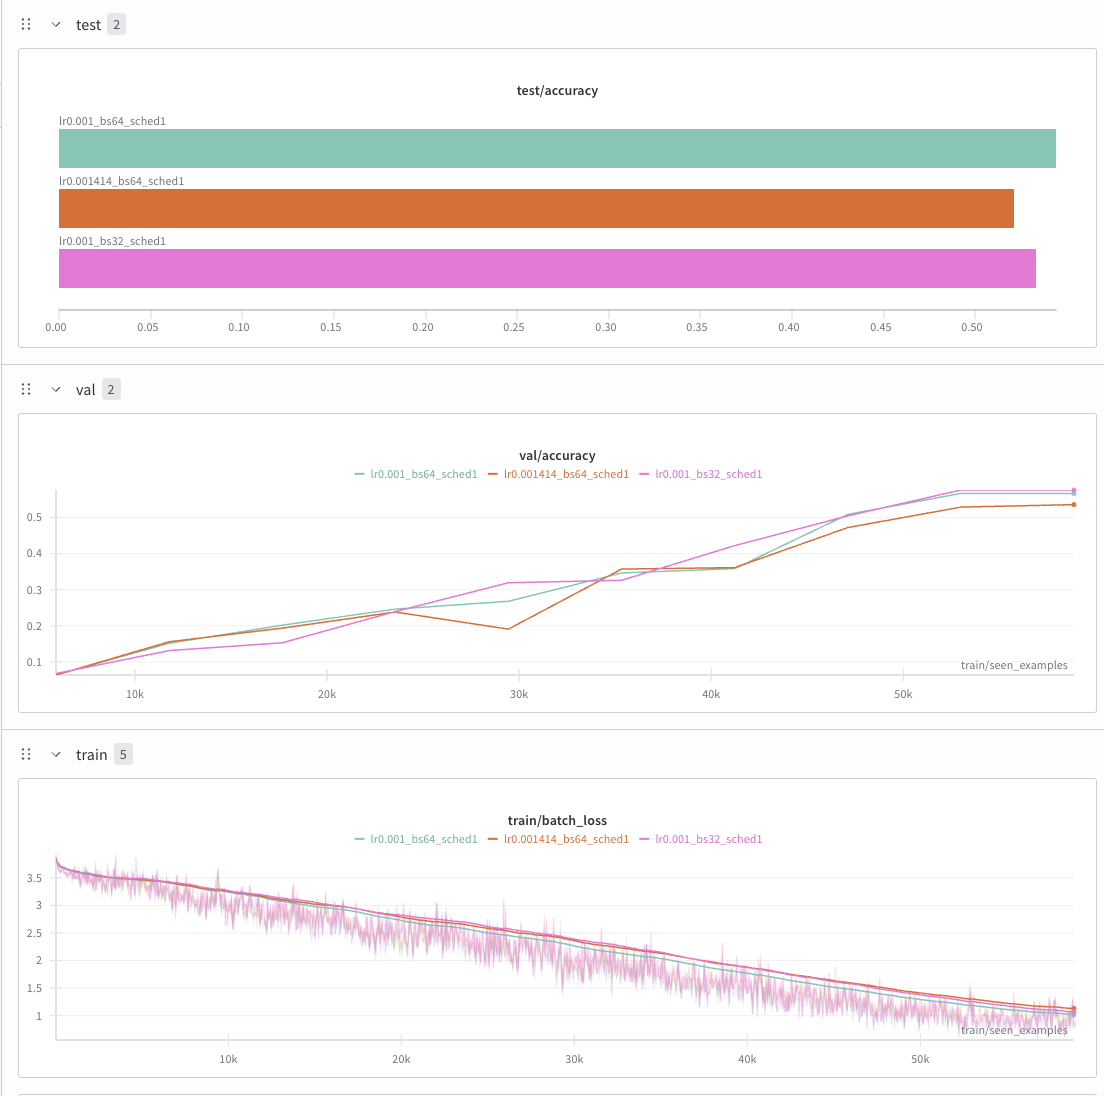
\includegraphics[width=0.8\textwidth]{images/batch_size_scheduler.png}
    \caption{Batch Size with Scheduler}
\end{figure}

\end{answerbox}

\subsection*{Part 4: Fine-Tuning a Pretrained Model (3 points)}
Fine-tuning leverages the knowledge of models trained on large datasets by adapting their weights to a new task. In this section, you will fine-tune a ResNet-18 model pre-trained on ImageNet using \texttt{torchvision.models.resnet18(pretrained=True)}. Modify the classification head to match the number of classes in your task, and replace the model definition in the original code. Keep the rest of the setup as default for comparison.


\noindent\textbf{Deliverable:}
\begin{itemize}
    \item Present charts showing: training loss, validation accuracy, and final test accuracy.
    \item Analyze the impact of pre-training on the model's learning process and performance.
    
\end{itemize}

\begin{answerbox} \textbf{Answer:} \vspace*{1cm}


Screenshot(s) of W\&B charts:

\begin{figure}[h]
    \centering
    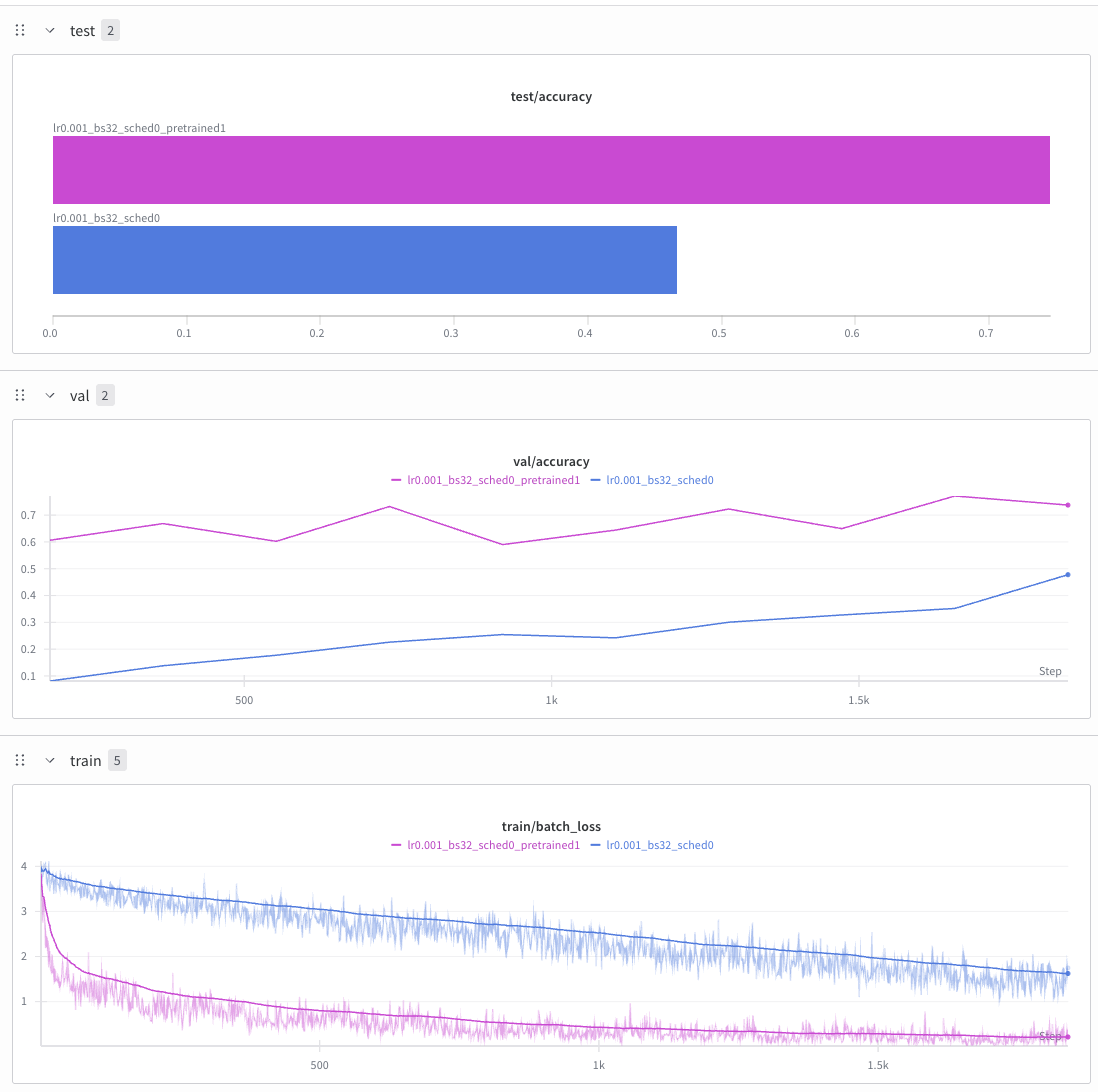
\includegraphics[width=0.8\textwidth]{images/pretrained.png}
    \caption{Pretrained Model}
\end{figure}

Pre-training allows the model to converge to a relatively better position at the beginning of training, making the subsequent training process more stable and resulting in higher final accuracy.

\end{answerbox}


\clearpage

\section*{Problem 2 - Model Testing}
Unlike model evaluation, which focuses on performance metrics, model testing ensures that a model behaves as expected under specific conditions.

\begin{itemize}
    \item \textbf{Pre-Train Test:} Conducted before training, these tests identify potential issues in the model's architecture, data preprocessing, or other components, preventing wasted resources on flawed training.
    \item \textbf{Post-Train Test:} Performed after training, these tests evaluate the model's behavior across various scenarios to ensure it generalizes well and performs as expected in real-world situations.
    
\end{itemize}

In this problem, you will examine the code and model left by a former employee who displayed a lack of responsibility in his work. The code can be found in the \texttt{Problem 2} folder. The necessary predefined functions for this task are available in the \texttt{model\_testing.py} file. Follow the instructions provided in that file for detailed guidance.

\subsection*{Part 1: Pre-Train Testing}

In this part, you will apply pre-train tests to verify experimental correctness before training is conducted. \noindent\textbf{Deliverables:} For each question in Part 1, provide clear deliverables of the following:
\begin{enumerate}
    \item Observations and analysis of the results.
    \item Suggested approaches for addressing the detected issues (if any).
    \item Code implementation.
\end{enumerate}

\subsubsection*{Data Leakage Check (3 points)}
Load the training, validation, and test data sets using \texttt{get\_dataset()} function. Check for potential data leakage between these sets by directly comparing the images, as data augmentation was not applied. Since identical objects usually have different hash values in Python, consider using techniques like image hashing for this comparison.

\begin{answerbox} \textbf{Answer:} \vspace*{1cm}

1. Observations and analysis of the results.
    All of the images in the test set are also in the train set.
2. Suggested approaches for addressing the detected issues (if any).
    I think we should remove the images that are in the test set from the train set.
3. Code implementation.

\begin{verbatim}
from utils.datasets import get_dataset
train_dataset, val_dataset, test_dataset = get_dataset()

logging.basicConfig(level=logging.INFO, format="%(asctime)s - %(levelname)s - %(message)s")


def tensor_to_bytes(image_tensor: torch.Tensor) -> bytes:
    detached_tensor = image_tensor.detach().cpu()
    numpy_tensor = np.asarray(detached_tensor)
    return numpy_tensor.tobytes()


def build_hash_catalog(dataset, dataset_name):
    logging.info("Hashing %s dataset with %d samples", dataset_name, len(dataset))
    dataset_hash_catalog = {}
    for sample_index in range(len(dataset)):
        image_tensor, _ = dataset[sample_index]
        content_bytes = tensor_to_bytes(image_tensor)
        sample_hash = hashlib.sha256(content_bytes).hexdigest()
        dataset_hash_catalog.setdefault(sample_hash, []).append(sample_index)
    logging.info("Completed hashing %s dataset", dataset_name)
    return dataset_hash_catalog


def report_dataset_overlap(primary_catalog, secondary_catalog, primary_name, secondary_name):
    overlapping_hashes = set(primary_catalog.keys()).intersection(secondary_catalog.keys())
    logging.info(
        "Detected %d overlapping images between %s and %s",
        len(overlapping_hashes),
        primary_name,
        secondary_name,
    )
    return overlapping_hashes


train_hash_catalog = build_hash_catalog(train_dataset, "train")
validation_hash_catalog = build_hash_catalog(val_dataset, "validation")
test_hash_catalog = build_hash_catalog(test_dataset, "test")

overlap_train_validation = report_dataset_overlap(
    train_hash_catalog,
    validation_hash_catalog,
    "train",
    "validation",
)
overlap_train_test = report_dataset_overlap(
    train_hash_catalog,
    test_hash_catalog,
    "train",
    "test",
)
overlap_validation_test = report_dataset_overlap(
    validation_hash_catalog,
    test_hash_catalog,
    "validation",
    "test",
)
print(len(train_dataset))
# remove the detected overlapping images from the train set
Non_overlap_indices = [
    indice
    for key, indice in train_hash_catalog.items()
    if key not in overlap_train_test
]
train_dataset = torch.utils.data.Subset(train_dataset, Non_overlap_indices)
print(len(train_dataset))

\end{verbatim}

\end{answerbox}

\subsubsection*{Model Architecture Check (2 points)}
Initialize the model using the \texttt{get\_model()} function. Verify that the model’s output shape matches the label format (hint: consider the number of classes in the dataset).

\begin{answerbox} \textbf{Answer:} \vspace*{1cm}


1. Observations and analysis of the results.
    The model's output shape 128 does not match the label format which is 10.
2. Suggested approaches for addressing the detected issues (if any).
    I think we should remove the last layer of the model so that the output shape matches the label format since the shape of the output of fc1 is 10:
    (fc1): Linear(in_features=2048, out_features=10, bias=True)
    (fc2): Linear(in_features=10, out_features=128, bias=True)
3. Code implementation.

\begin{verbatim}
from utils.models import get_model
model = get_model()
model.eval()

base_dataset = train_dataset.datasets[0]
expected_class_count = len(base_dataset.classes)
verification_loader = DataLoader(train_dataset, batch_size=32)
sample_images, sample_labels = next(iter(verification_loader))
with torch.no_grad():
    output_tensor = model(sample_images)

output_feature_count = output_tensor.shape[-1]

logging.info("Model output feature count: %d", output_feature_count)
logging.info("Expected class count: %d", expected_class_count)

if output_feature_count == expected_class_count:
    logging.info("Model output shape matches label format.")
else:
    logging.warning(
        "Model output feature count %d does not match label class count %d.",
        output_feature_count,
        expected_class_count,
    )

# remove the last layer of the model
model.fc2 = nn.Identity()

# test the model
with torch.no_grad():
    output_tensor = model(sample_images)
    print(output_tensor.shape)    
\end{verbatim}
\end{answerbox} 

\subsubsection*{Gradient Descent Validation (2 points)}
Verify that ALL the model's trainable parameters are updated after a single gradient step on a batch of data.

\begin{answerbox} \textbf{Answer:} \vspace*{1cm}
1. Observations and analysis of the results.
    There are many downsample layers which do not update parameters.
2. Suggested approaches for addressing the detected issues (if any).
    I don't know. I checked that all of the parameters require grad. I have never seen this problem before.
3. Code implementation.
\begin{verbatim}
    from torch.optim import AdamW
    from torch.nn import CrossEntropyLoss
    
    trainable_params = [p for p in model.parameters() if p.requires_grad]
    optimizer = torch.optim.SGD(trainable_params, lr=1e-2, momentum=0.9, weight_decay=0)
    train_loader = DataLoader(train_dataset, batch_size=32)
    criterion = CrossEntropyLoss()
    model.train()
    initial_parameter_state = {}
    for parameter_name, parameter_tensor in model.named_parameters():
        if parameter_tensor.requires_grad:
            initial_parameter_state[parameter_name] = (
                parameter_tensor.detach().cpu().clone()
            )
    step_images, step_labels = next(iter(train_loader))
    optimizer.zero_grad(set_to_none=True)
    predicted_logits = model(step_images)
    step_loss = criterion(predicted_logits, step_labels)
    step_loss.backward()
    optimizer.step()
    
    static_parameters = []
    for parameter_name, parameter_tensor in model.named_parameters():
        if parameter_tensor.requires_grad:
            previous_tensor = initial_parameter_state[parameter_name]
            if torch.allclose(
                previous_tensor, parameter_tensor.detach().cpu(), rtol=1e-7, atol=1e-9
            ):
                static_parameters.append(parameter_name)
    
    if static_parameters:
        logging.warning("Parameters unchanged after gradient step: %s", static_parameters)
    else:
        logging.info("All trainable parameters updated after the gradient step.")
\end{verbatim}
\end{answerbox}


\subsubsection*{Learning Rate Check (2 points)}
 Implement the learning rate range test using \href{https://github.com/davidtvs/pytorch-lr-finder#tweaked-version-from-fastaiauto}{pytorch-lr-finder}. Determine whether the learning rate is appropriately set by examining the loss-learning rate graph. Necessary components for \texttt{torch\_lr\_finder.LRFinder} are provided in \texttt{model\_testing.py}.


\begin{answerbox} \textbf{Answer:} \vspace*{1cm}

1. Observations and analysis of the results.
\begin{figure}[h]
    \centering
    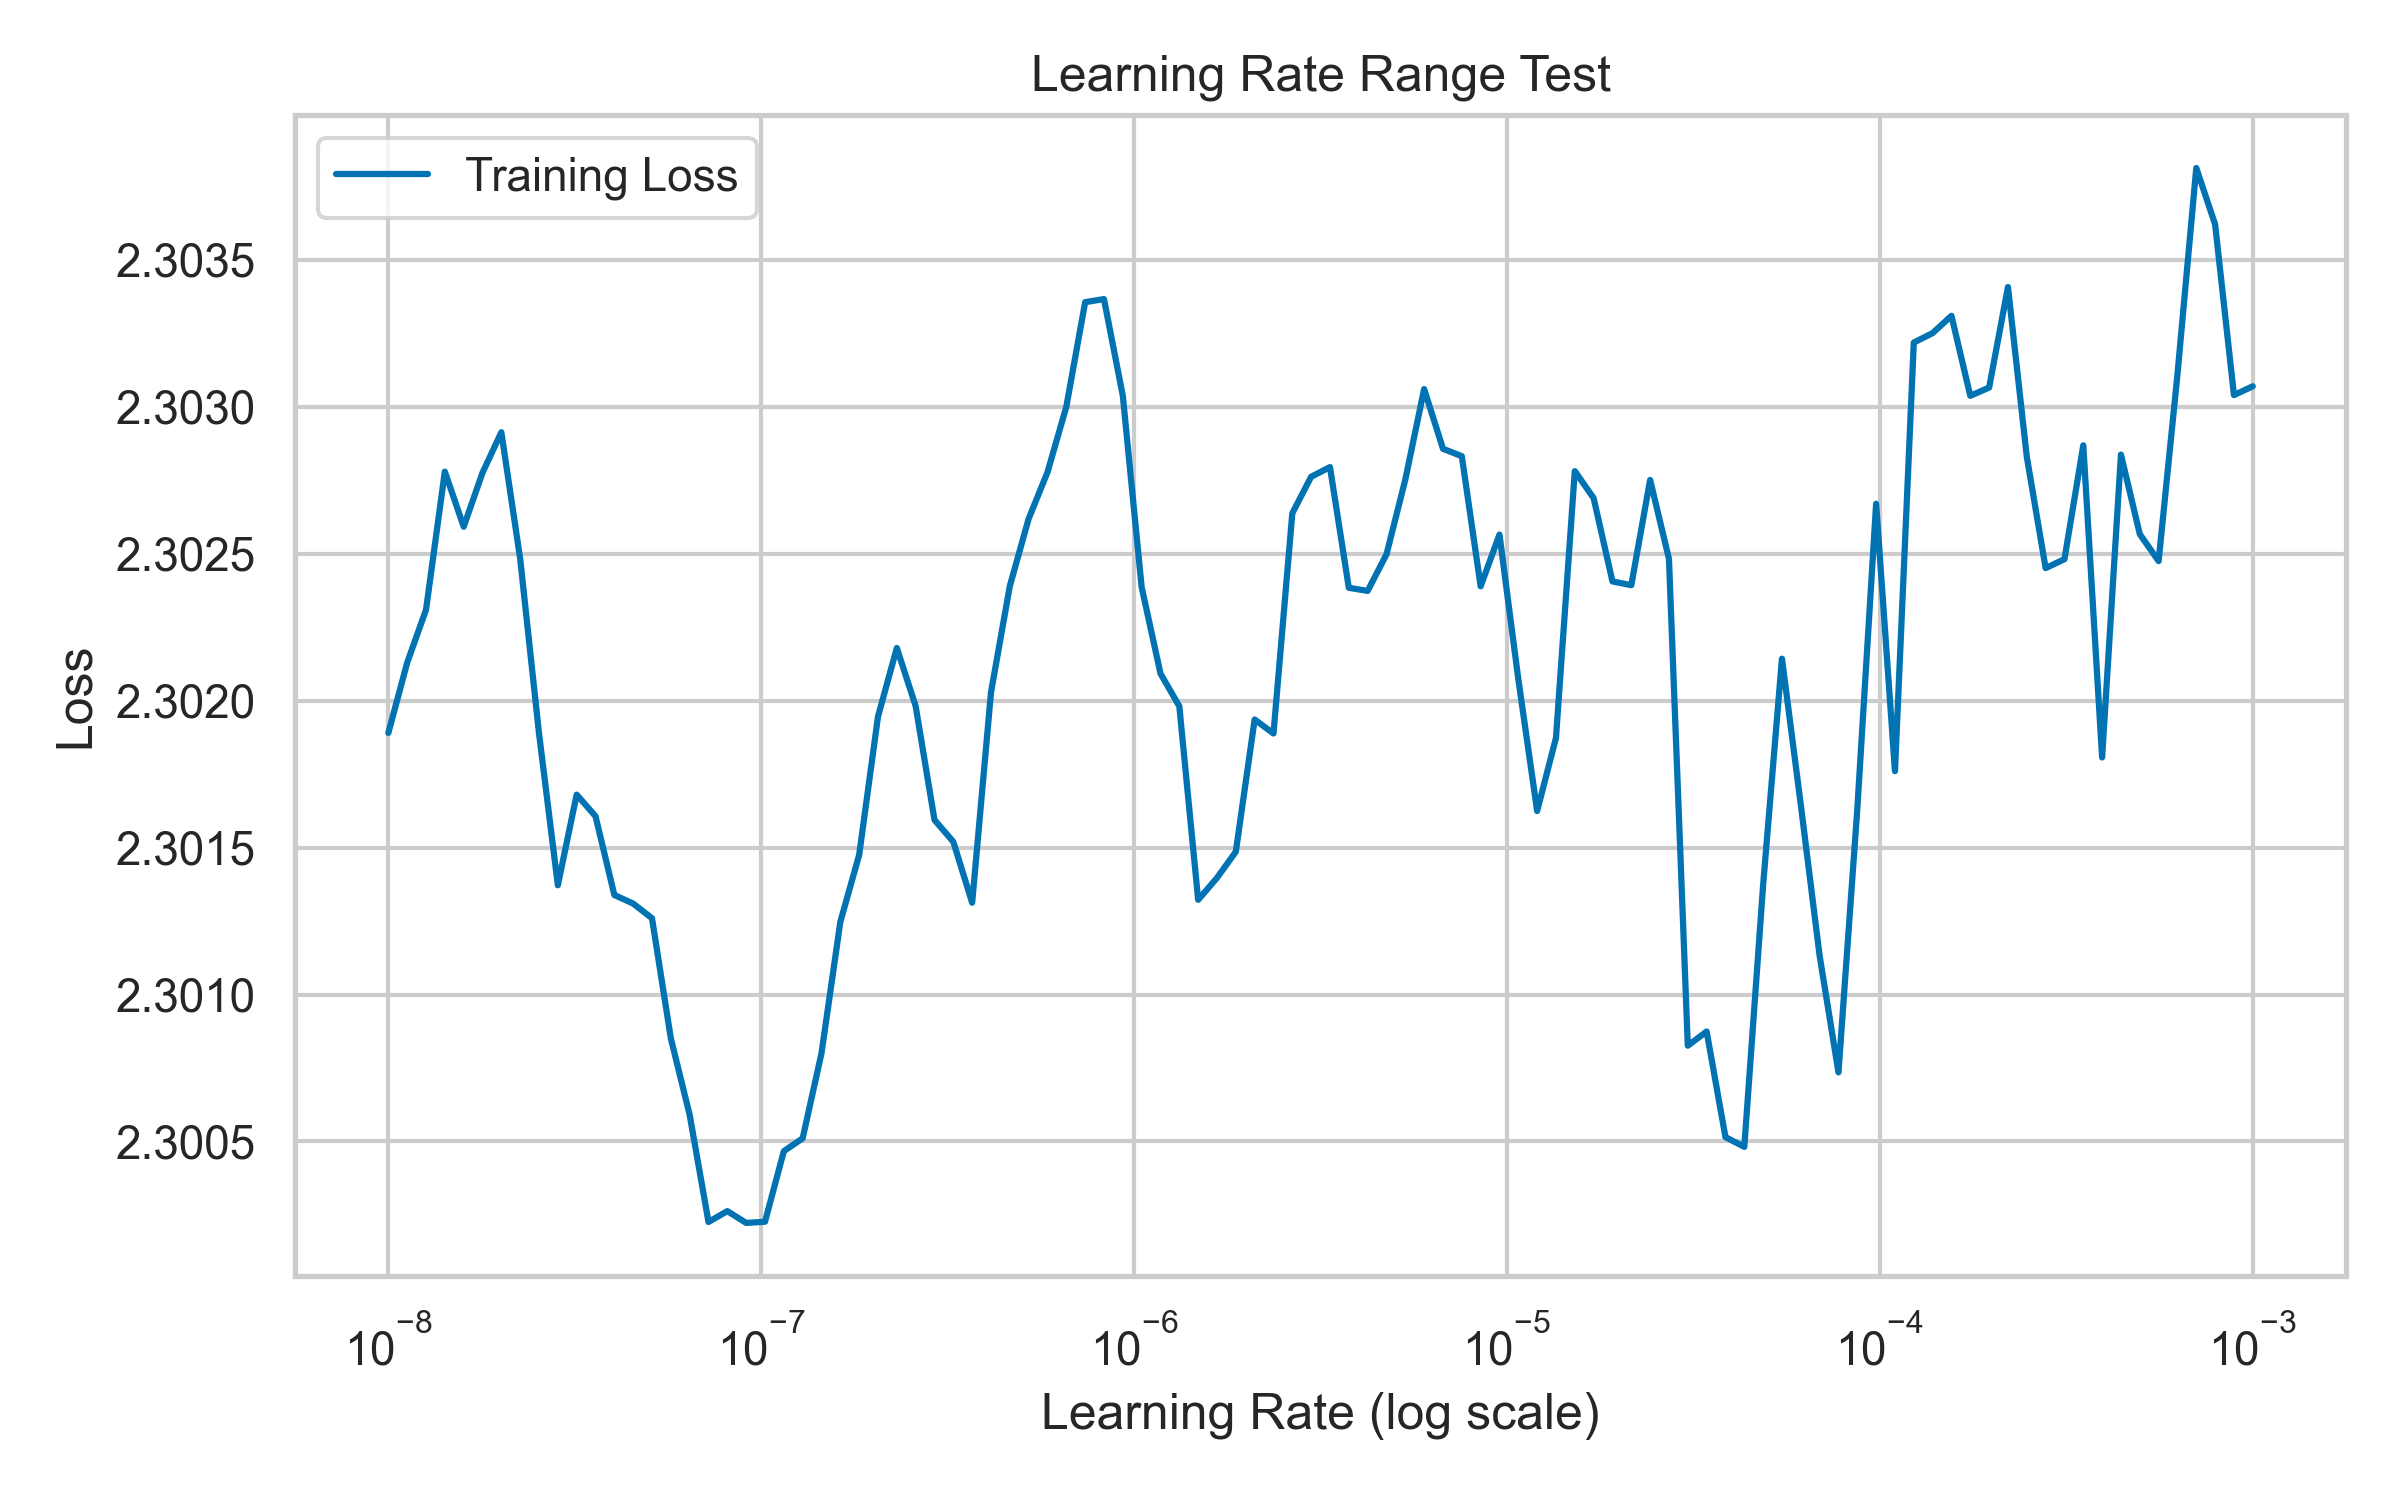
\includegraphics[width=0.8\textwidth]{problem_2/outputs/learning_rate_range_test.png}
    \caption{Learning Rate Check}
\end{figure}
\end{answerbox}

It seems that the best learning rate is between 1e-5 and 1e-4, and 1e-6 is not the best.

2. Suggested approaches for addressing the detected issues (if any).
    I think we should set the learning rate to 5e-5.
3. Code implementation.
\begin{verbatim}
    from torch.optim import AdamW
    from torch.nn import CrossEntropyLoss
    from torch_lr_finder import LRFinder
    
    optimizer = AdamW(
        model.parameters(), lr=1e-6
    )  # the lr is set to 1e-6 as specified here
    criterion = CrossEntropyLoss()
    train_loader = verification_loader
    configured_learning_rate = optimizer.param_groups[0]["lr"]
    
    logging.info("Starting learning rate range test with torch_lr_finder.")
    original_training_mode = model.training
    model.train()
    
    
    target_iterations = min(len(train_loader), 100)
    device = next(model.parameters()).device
    lr_finder = LRFinder(model, optimizer, criterion, device=device)
    lr_finder.range_test(
        train_loader,
        start_lr=1e-8,
        end_lr=1e-3,
        num_iter=target_iterations,
        step_mode="exp",
    )
    history_frame = pl.DataFrame(
        {
            "learning_rate": lr_finder.history["lr"][:target_iterations],
            "loss": lr_finder.history["loss"][:target_iterations],
        }
    )
    sns.set_theme(style="whitegrid", palette="colorblind")
    figure, axis = plt.subplots(figsize=(8, 5))
    sns.lineplot(
        data=history_frame.to_pandas(),
        x="learning_rate",
        y="loss",
        ax=axis,
        label="Training Loss",
    )
    axis.set_xscale("log")
    axis.set_title("Learning Rate Range Test")
    axis.set_xlabel("Learning Rate (log scale)")
    axis.set_ylabel("Loss")
    axis.legend(loc="best")
    figure.tight_layout()
    output_directory = Path("problem_2") / "outputs"
    output_directory.mkdir(parents=True, exist_ok=True)
    plot_path = output_directory / "learning_rate_range_test.png"
    figure.savefig(plot_path, dpi=300)
    logging.info("Learning rate range test plot saved to %s", plot_path)
    plt.close(figure)
    search_start_index = min(5, target_iterations - 1)
    search_window_size = target_iterations - search_start_index
    if search_window_size <= 0:
        best_lr_record = history_frame.row(target_iterations - 1, named=True)
    else:
        best_lr_record = (
            history_frame.slice(search_start_index, search_window_size)
            .sort("loss")
            .row(0, named=True)
        )
    suggested_learning_rate = float(best_lr_record["learning_rate"])
    lowest_observed_loss = float(best_lr_record["loss"])
    logging.info(
        "Lowest observed loss %.4f occurred at learning rate %.2e during range test.",
        lowest_observed_loss,
        suggested_learning_rate,
    )
    logging.info("Suggested learning rate: %f", suggested_learning_rate)
    logging.info("Configured learning rate: %f", configured_learning_rate)
    lr_finder.reset()
\end{verbatim}

\subsection*{Part 2: Post-Train Testing}

\subsubsection*{Dying ReLU Examination (4 points)}
In this section, you will examine the trained model for ``Dying ReLU." \href{https://datascience.stackexchange.com/questions/5706/what-is-the-dying-relu-problem-in-neural-networks}{Dying ReLU} occurs when a ReLU neuron outputs zero consistently and cannot differentiate between inputs. 
Load the trained model using \texttt{get\_trained\_model()} function, and the test set using \texttt{get\_test\_set()} function. Review the model's architecture, which is based on ResNet and can be found in \texttt{utils/trained\_models.py}. Then address the following:


\begin{enumerate}
    \item Identify the layer(s) where Dying ReLU might occur and explain why.
    \item Describe your approach for detecting Dying ReLU neurons. 
    \item Determine if Dying ReLU neurons are present in the trained model, and provide your code implementation..
\end{enumerate}
\textbf{Hint}: Consider how BatchNorm operation would influence the presence of dying ReLU.
    
\begin{answerbox} \textbf{Answer:} \vspace*{1cm}

\end{answerbox}

\subsubsection*{Model Robustness Test - Brightness (4 points)}
In this section, you will evaluate the model's robustness to changes in image brightness using a defined brightness factor.
Define a brightness factor $\lambda$, which determines the image brightness by multiplying pixel values by $\lambda$. Specifically, $\lambda = 1$ corresponds to the original image's brightness.
Load the trained model using \texttt{get\_trained\_model()} function, and the test dataset using \texttt{get\_test\_set()} function.  Investigate the model's performance across various brightness levels by adjusting $\lambda$ from $0.2$ to $1.0$ in increments of $0.2$. 

\noindent\textbf{Deliverable:}

\begin{enumerate}
    \item  Plot a curve showing how model accuracy varies with brightness levels.
    \item Analyze the relationship and discuss any trends observed.
\end{enumerate}


\begin{answerbox} \textbf{Answer:} \vspace*{1cm}

\end{answerbox}


\subsubsection*{Model Robustness Test - Rotation (4 points)}

Evaluate the model's robustness to changes in image rotation. Rotate the input image from $0$ to $300$ degrees in increments of $60$ degrees. 
Similarly, load the trained model using \texttt{get\_trained\_model()} function, and the test set using \texttt{get\_test\_set()} function. 

\noindent\textbf{Deliverable:}

\begin{enumerate}
    \item Plot a curve showing the relationship between rotation angles and model accuracy.
    \item Analyze the trend and discuss any observed patterns.
    \item Suggest potential improvements to enhance model robustness
\end{enumerate}



\begin{answerbox} \textbf{Answer:} \vspace*{1cm}

\end{answerbox}


\subsubsection*{Normalization Mismatch (2 points)}

Load the test set using the \texttt{get\_test\_set()} function. Assume that the mean and standard deviation (std) used to normalize the testing data are different from those applied to the training data.

\noindent\textbf{Deliverable:}

\begin{enumerate} \item Calculate and report the mean and std of the images in the loaded test set (\href{https://stackoverflow.com/questions/73350133/how-to-calculate-mean-and-standard-deviation-of-a-set-of-images}{tutorial}). Compare these values with the expected mean and std after proper normalization.

\item Discuss one potential impact of this incorrect normalization on the model's performance or predictions. 

\end{enumerate}

\begin{answerbox} \textbf{Answer:} \vspace*{1cm}


\end{answerbox}


\end{document}  